The CQT Post Processor (CQTPP) was first introduced by the CQTech team during the ORCA Hackathon. It addresses both bias and autocorrelation reduction in randomly generated numbers that may be biased and correlated (or dependent), unlike the Von Neumann method, which requires the input to be uniformly biased and independent.

The CQTPP algorithm (detailed in the appendices) follows these steps:

\begin{enumerate}
    \item \textbf{Divide the input bitstream} into two equal samples: Sample 1 and Sample 2.
    \item \textbf{Divide each sample into chunks} of a pre-defined size, referred to as the \texttt{dep\_seq\_len} (a hyperparameter).
    \item \textbf{Process the chunks as follows:}
    \begin{itemize}
        \item Take the first chunk from Sample 1 and the first chunk from Sample 2.
        \item For each pair of chunks, take the corresponding bits from both chunks and apply the \textbf{Von Neumann mapping}.
        \item Continue this process until all bits in the chunks are processed (the size of each chunk is \texttt{dep\_seq\_len}).
    \end{itemize}
    \item \textbf{For each pair of chunks}, obtain the Von Neumann processed output.
    \item \textbf{Take only the first bit} of that output and append it to the final result of CQTPP, discarding the remaining bits.
    \item \textbf{Repeat this operation} for all remaining chunks.
\end{enumerate}

This process is illustrated in \textbf{Fig. \ref{fig:CQTPP_process}}.

\begin{figure}[h]
\centering
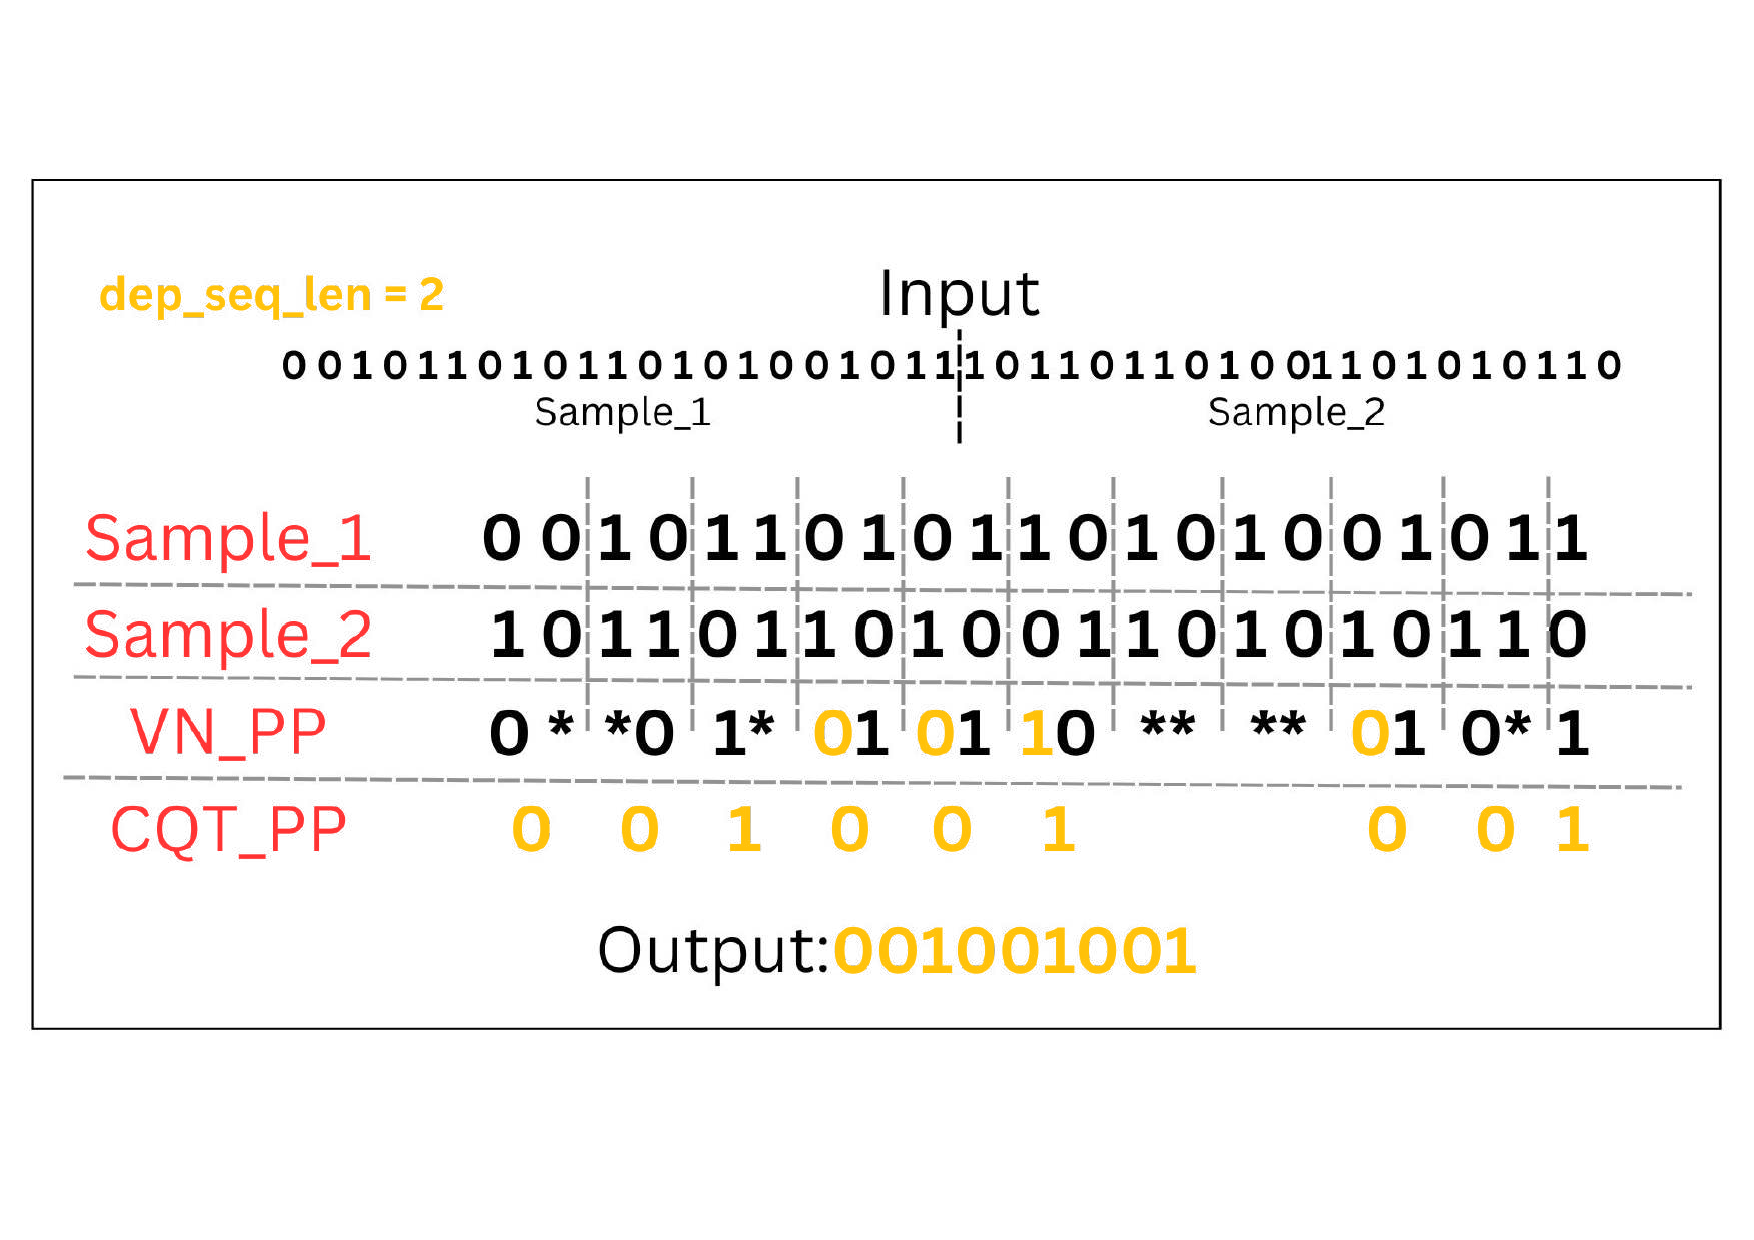
\includegraphics[width=12cm]{figures/CQTPP.pdf}
\caption{Diagram illustrating the process of the CQT Post Processor (CQTPP)}
\label{fig:CQTPP_process}
\end{figure}

\section{Performance and Output Results}

Considering we have a bitstream of length 4, all possible combinations are \(2^4 = 16\). Table~\ref{tab:output_comparison} shows the outputs generated using both the CQT Post Processor (CQTPP) and the Von Neumann Post Processor (VonNeuPP).

\begin{table}[h]
\centering
\caption{Output Comparison Between CQTPP and VonNeuPP}
\label{tab:output_comparison}
\begin{tabular}{|c|c|c|}
\hline
\textbf{Bits} & \textbf{CQTPP Output} & \textbf{VonNeuPP Output} \\ \hline
0000 & X  & X  \\ \hline
0001 & 0  & 0  \\ \hline
0010 & 0  & 0  \\ \hline
0011 & 0  & 00 \\ \hline
0100 & 1  & 1  \\ \hline
0101 & X  & X  \\ \hline
0110 & 0  & 01 \\ \hline
0111 & 0  & 0  \\ \hline
1000 & 1  & 1  \\ \hline
1001 & 1  & 10 \\ \hline
1010 & X  & X  \\ \hline
1011 & 0  & 0  \\ \hline
1100 & 1  & 11 \\ \hline
1101 & 1  & 1  \\ \hline
1110 & 1  & 1  \\ \hline
1111 & X  & X  \\ \hline
\end{tabular}
\end{table}

In the table, \(X\) indicates no output.

As mentioned in previous sections, for a number to be truly random, the probabilities of obtaining a 0 or 1 should be equal. Additionally, the probabilities of obtaining the bit pairs \(00\), \(01\), \(10\), and \(11\) should also be equal.

Let \(p_{00}\), \(p_{01}\), \(p_{10}\), and \(p_{11}\) denote the probabilities that the input bitstream contains the respective pairs \(00\), \(01\), \(10\), and \(11\). For example, the probability that the input bitstream is \(0110\) is given by:
\[
p(\text{0110}) = p_{01} \times p_{10}
\]

To prove the unbiasedness of the output, we need to show that:
\[
p(\text{out} = 0) = p(\text{out} = 1)
\]
and also:
\[
p(\text{out} = 00) = p(\text{out} = 01) = p(\text{out} = 10) = p(\text{out} = 11)
\]

\noindent As proven in the appendix, for the Von Neumann Post Processor:
\[
p(\text{out} = 0) = p(\text{out} = 1)
\]

However, regarding the equal probabilities of bit pairs, we can extract from Table~\ref{tab:output_comparison} the following relationships:

\[
p(\text{out} = 00) = p_{00} \times p_{11}, \quad p(\text{out} = 11) = p_{11} \times p_{00}
\]
\[
p(\text{out} = 01) = p_{01} \times p_{10}, \quad p(\text{out} = 10) = p_{10} \times p_{01}
\]

\noindent Therefore, for the condition to be true, we need to satisfy:
\[
p_{00} \times p_{11} = p_{01} \times p_{10}
\]

\noindent This condition remains true for uncorrelated input data.

\noindent On the other hand, the CQTPP ensures equal probabilities for all possible outputs.

Since the outcomes of CQTPP are only one bit in length, the output matches the Von Neumann Post Processor for 8 cases (excluding the empty output). As previously proven, these cases are equally distributed, and we refer to this probability as \(a\).

For the CQTPP to be unbiased, the following condition must hold:
\[
P(\text{out} = 0) = P(\text{out} = 1)
\]

We can express \(P(\text{out} = 0)\) as:
\[
P(\text{out} = 0) = a + p_{00} \times p_{11} + p_{01} \times p_{10}
\]

Similarly, for \(P(\text{out} = 1)\):
\[
P(\text{out} = 1) = a + p_{11} \times p_{00} + p_{10} \times p_{01}
\]

Therefore, we have:
\[
P(\text{out} = 0) = P(\text{out} = 1)
\]

This equality holds regardless of whether the input data is correlated or independent.

\noindent The same scheme can be extended to larger-scale inputs, with the unbiasedness being preserved.

\section{CQTPP Variants}
In this study, we propose several variants that utilize the same core principles of the CQTPP and aim to improve its results.

\subsection{Iterative CQTPP (ItCQTPP)}
The Iterative CQTPP (ItCQTPP) variant focuses on improving the throughput of the CQTPP by minimizing discarded bits.  
In this scheme, the discarded bits from the Von Neumann output (the remaining bits after applying the CQTPP) are gathered and re-processed through the CQTPP.  
This iterative process allows for a reduction in wasted information, thus slightly increasing the overall efficiency and throughput of the post-processing.  

An illustration of the Iterative CQTPP method is shown in Fig.~\ref{fig:itcqtpp}.

\begin{figure}[h!]
    \centering
    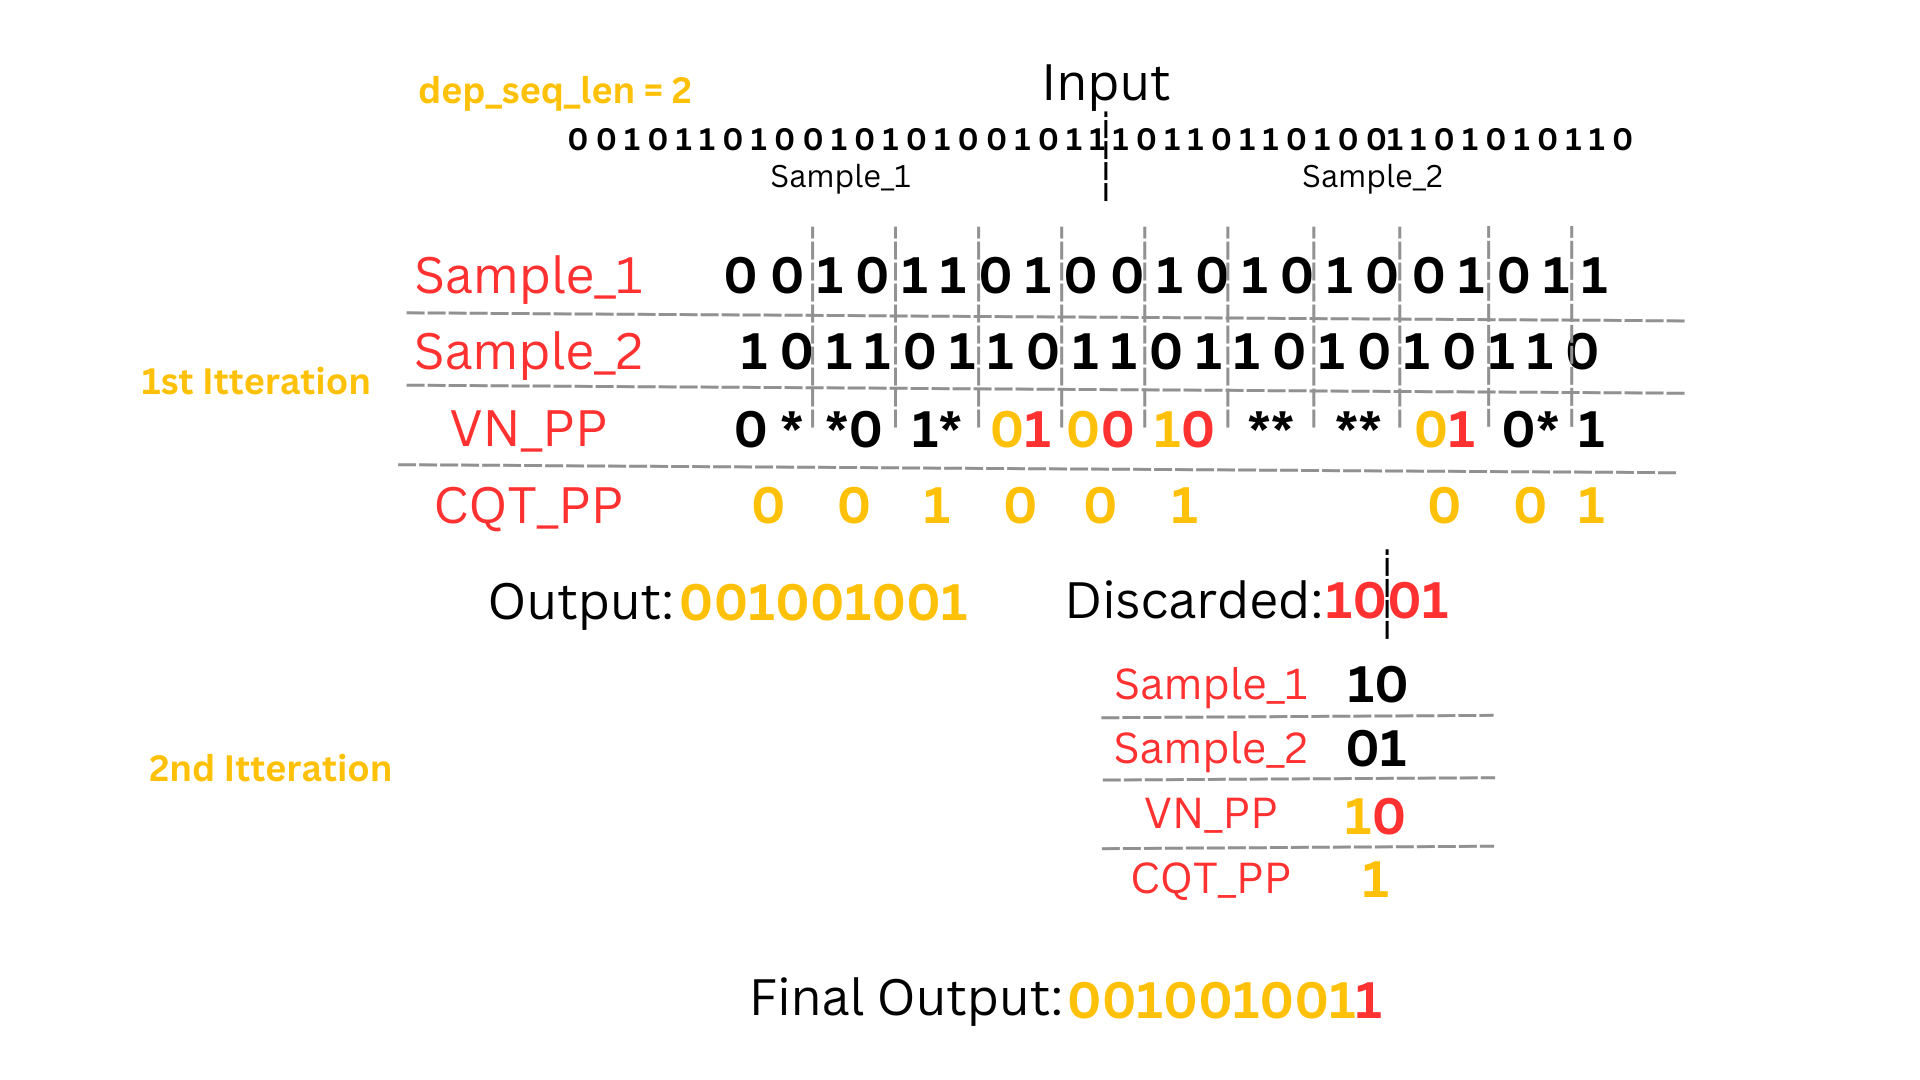
\includegraphics[width=0.8\textwidth]{figures/itcqtpp.png}
    \caption{Illustration of the process of the Iterative CQTPP method (ItCQTPP).}
    \label{fig:itcqtpp}
\end{figure}

\subsection{CQTPP/MKV}
The CQTPP/MKV variant aims to improve the de-correlation performance of the CQTPP by introducing a Markov Chain post-processing step.  
In this scheme, the output of the CQTPP is routed through a Markov Chain with either a 1-bit or 2-bit history.  
This additional step enhances the reduction of autocorrelation in the bitstream, leading to a more uniform and less predictable output.  

The schematic representation of the CQTPP/MKV method is shown in Fig.~\ref{fig:cqtppmkv}.



\begin{figure}[h!]
    \centering
    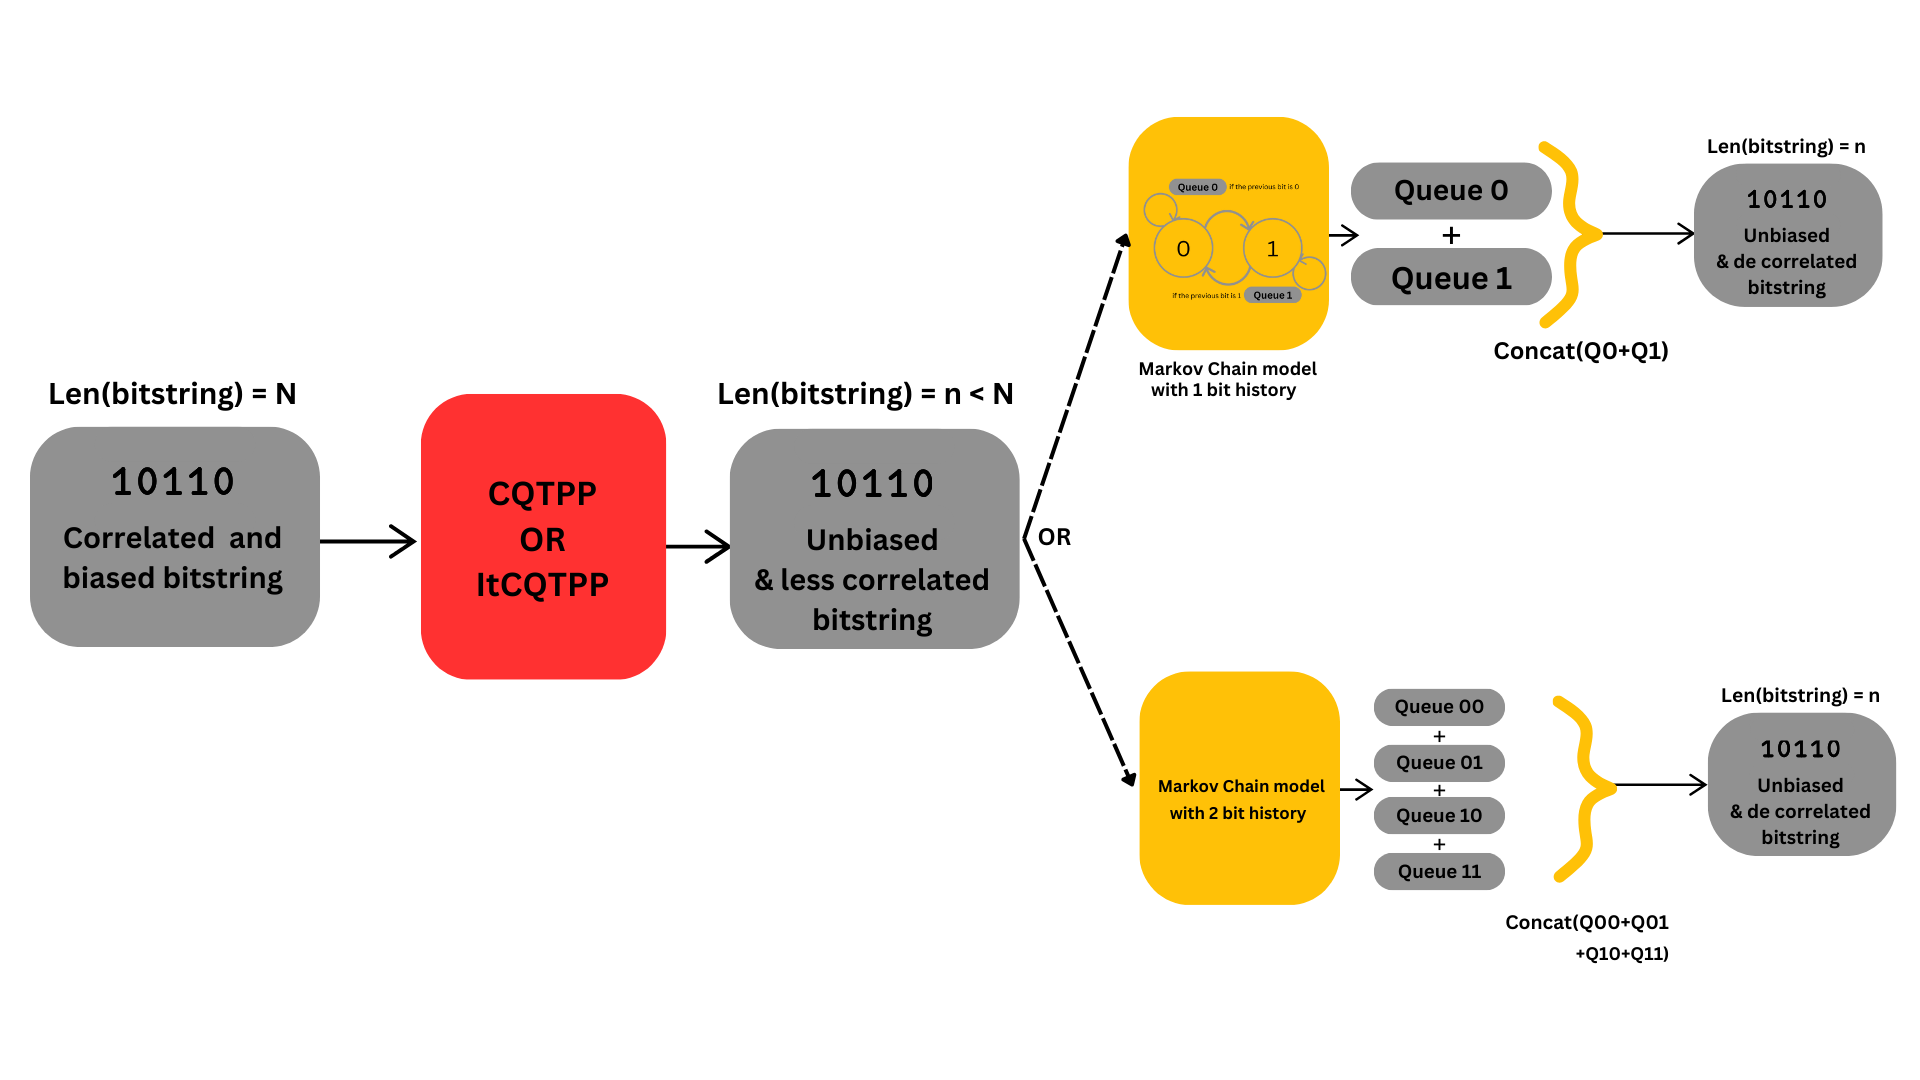
\includegraphics[width=0.8\textwidth]{figures/cqtppmkv.png}
    \caption{Schematic representation of the CQTPP/MKV method.}
    \label{fig:cqtppmkv}
\end{figure}



Now we are going to evaluate the results of the CQTPP and its variant based on the evaluation metrics we set above, and compare them with the Von Neumann Post Processors for different entropy sources sampling and using different hyper-parameters:

\subsection{The Entropy and n-bits Distribution}
Using a Markov model, we generated 20 bitstreams, each of length 10,000 (best for locally used computational power), by setting \( p_0 \), the probability that each bit is 0, and the autocorrelation coefficient \( \phi_1 \), which changes the nature of the entropy source as we can see in Table \ref{tab:experiments}.

\begin{table}[h!]
    \centering
    \begin{tabular}{|c|c|c|l|}
        \hline
        \textbf{Experiment} & \textbf{\( p_0 \)} & \textbf{Correlation Coefficient (\( \phi_1 \))} & \textbf{Remarks on the Nature} \\
        \hline
        A & 0.5 & 0 & Unbiased and independent \\
        B & 0.7 & 0 & Biased but independent \\
        C & 0.6 & 0.4 & Biased and autocorrelated \\
        D & 0.7 & 0.5 & Another biased and autocorrelated  \\
        \hline
    \end{tabular}
    \caption{Entropy source configurations for different experiments.}
    \label{tab:experiments}
\end{table}

The results are shown in Fig. \ref{fig:grph1}.

\begin{figure}[h!]
    \centering
    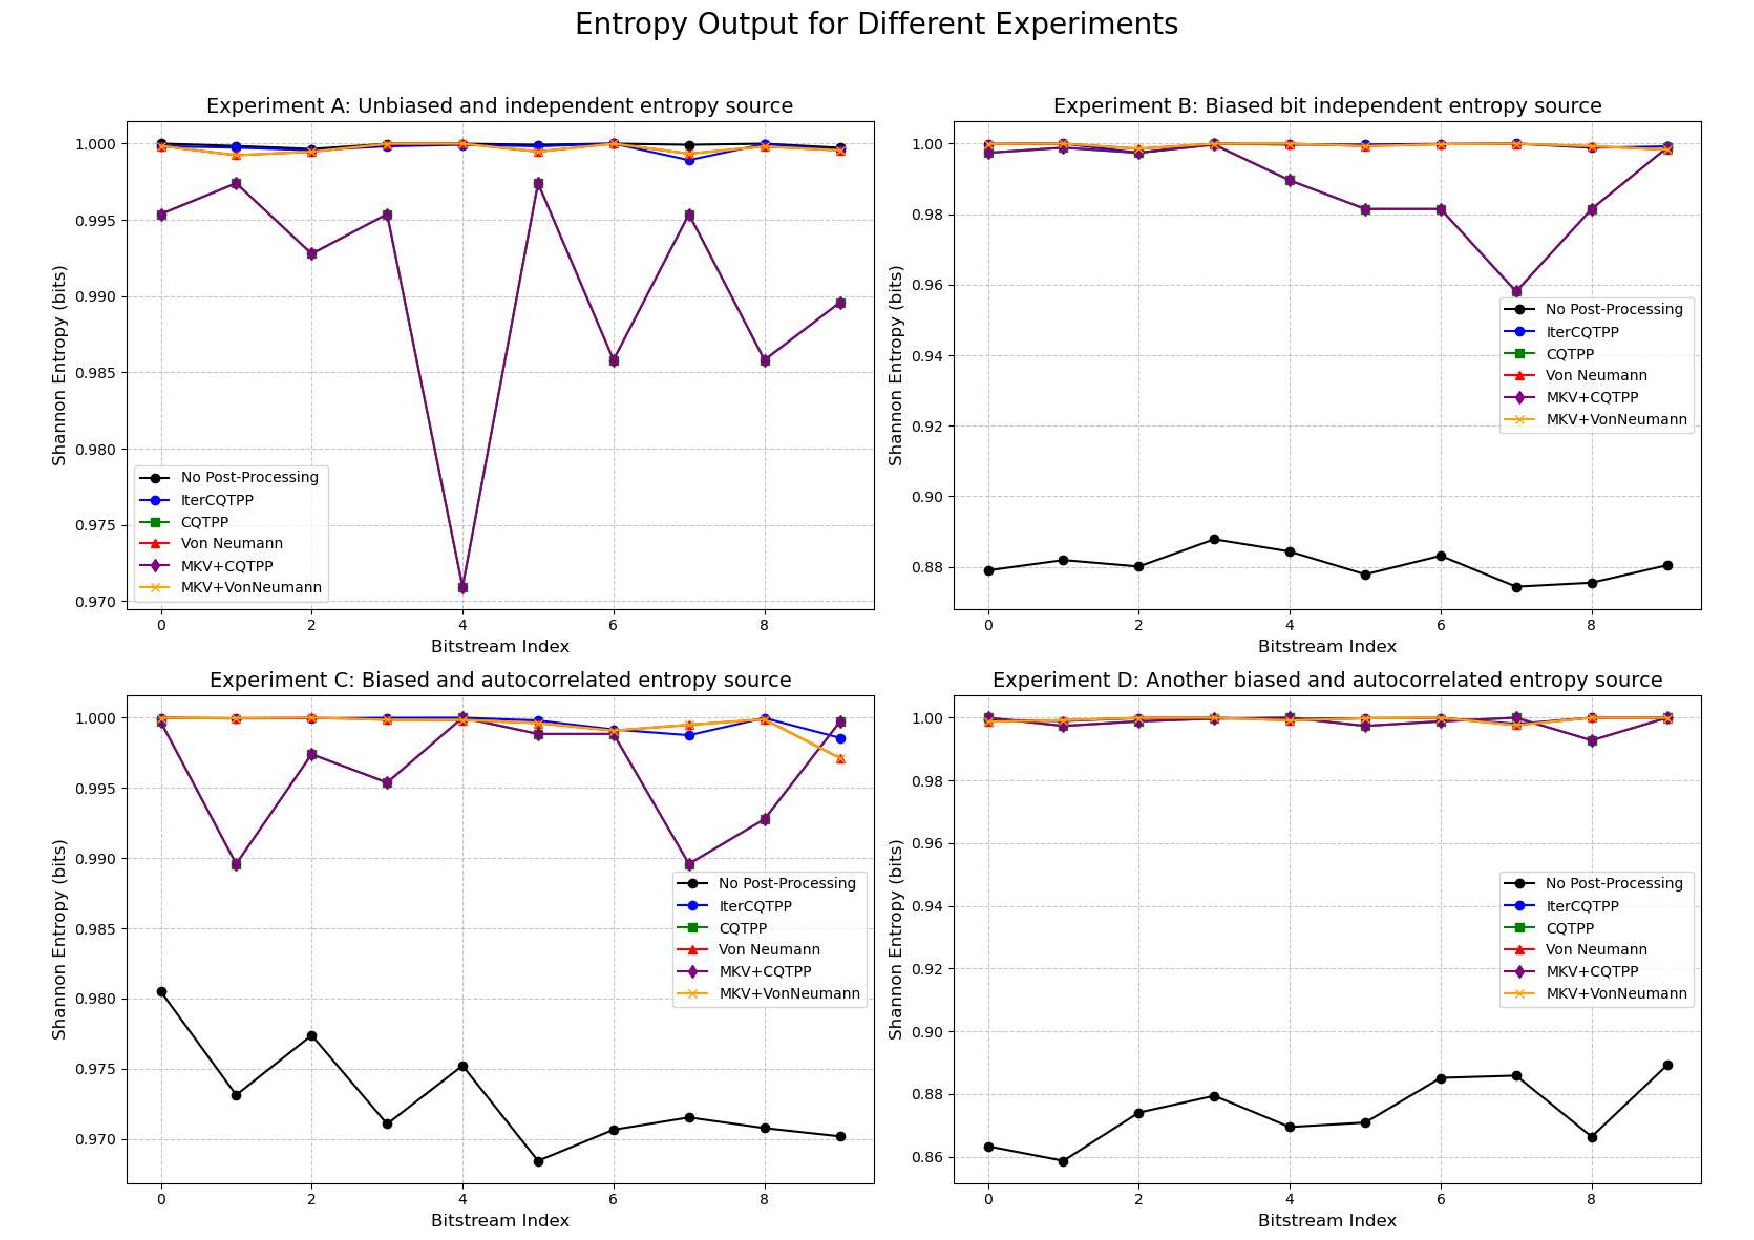
\includegraphics[width=\textwidth]{figures/download.pdf}
    \caption{Entropy output for different experiments using different post processors.}
    \label{fig:grph1}
\end{figure}

We can see that all the post processors and their variants performed well in increasing the entropy. The MKV+CQTPP shows some variance in results in the unbiased and independent bitstream, but it performed well in the other experiments when the autocorrelation increased.

Results distributions are shown in Fig. \ref{fig:grph2}.
Note: Reults will tend to be more unifrom whhen the bit length increases (we couldn't achieve that for computaional reasons)

\begin{figure}[h!]
    \centering
    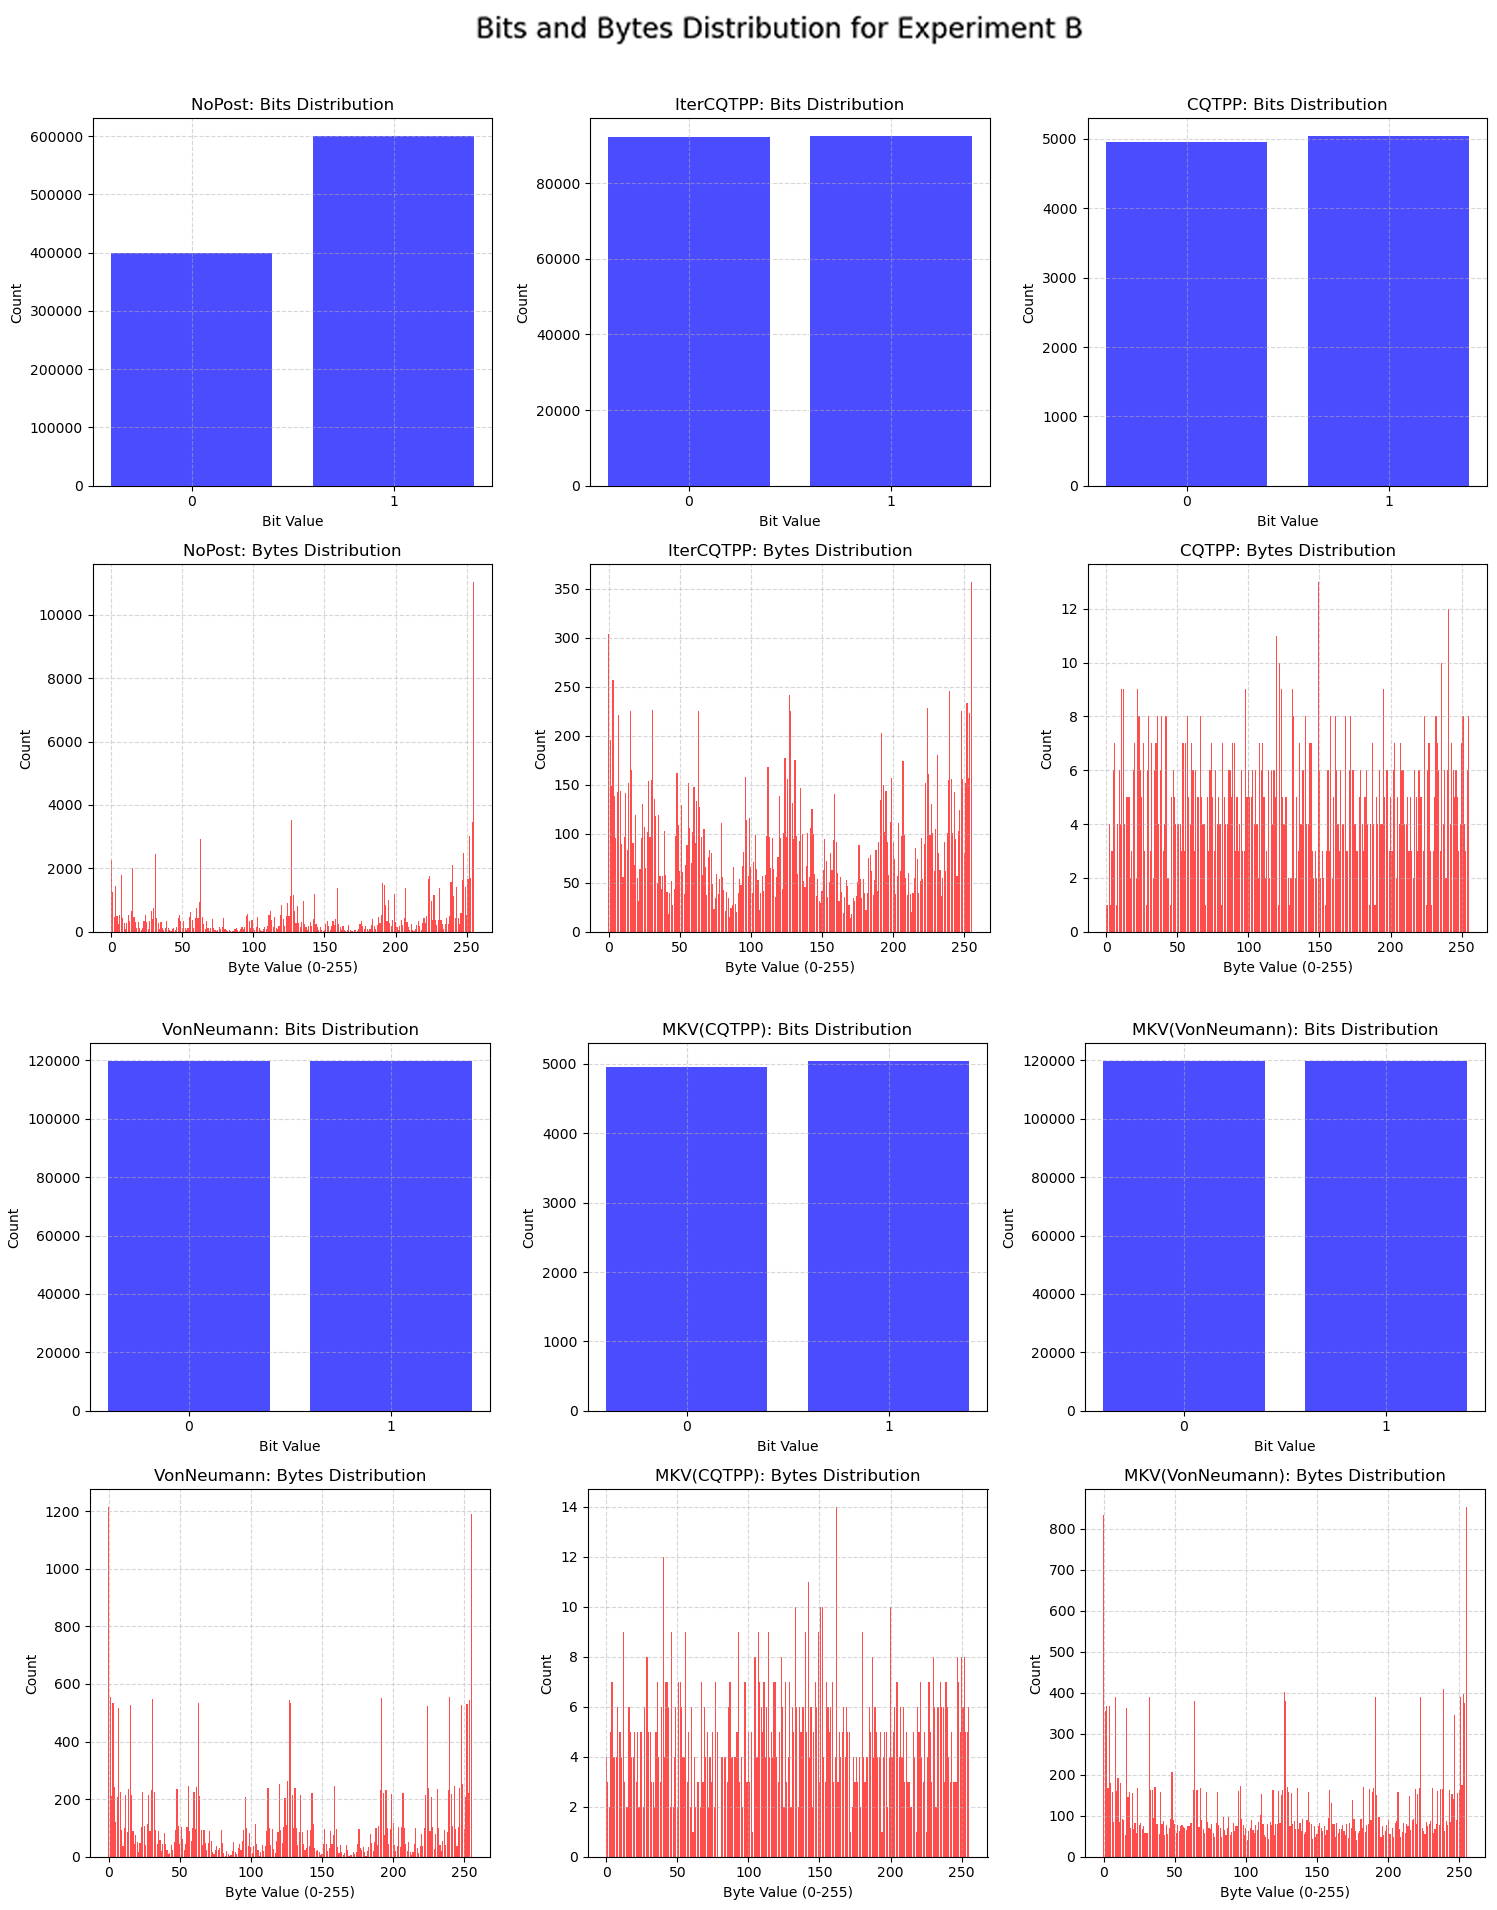
\includegraphics[width=\textwidth]{figures/ExperimentB Dists.png}
    \caption{Bits and Bytes Distribution Experiment C}
    \label{fig:grph2}
\end{figure}

We explore now the results with Real Borealis Data shared by Xanadu in \cite{data}

\noindent Results distributions are shown in Fig. \ref{fig:grph3}.

\begin{figure}[h!]
    \centering
    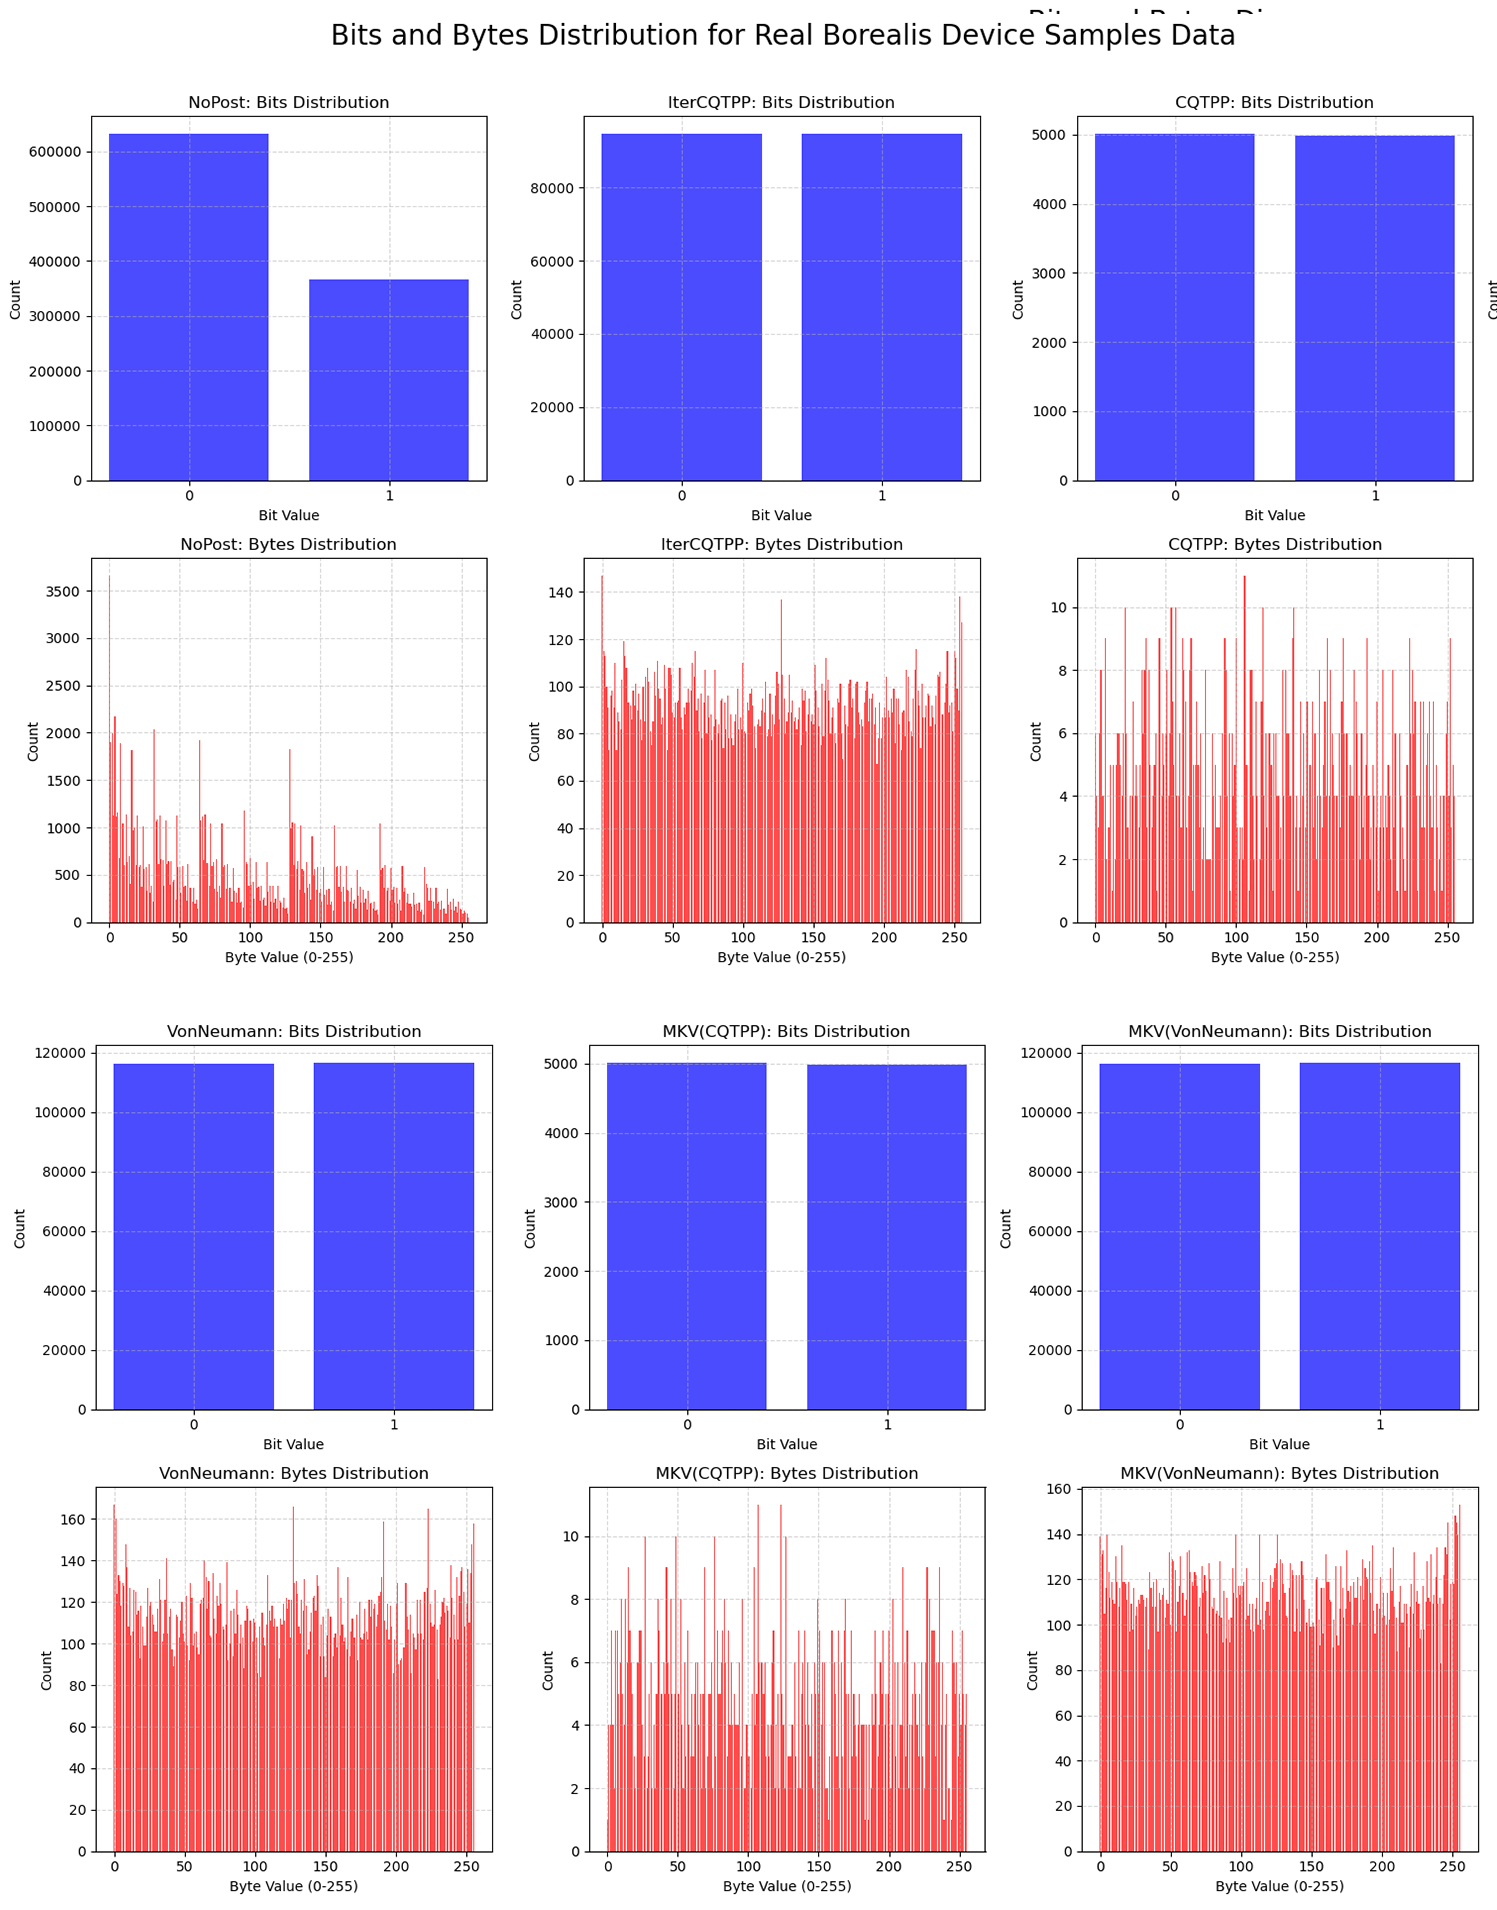
\includegraphics[width=\textwidth]{figures/BorealisResults Dist.png}
    \caption{Bits and Bytes Distribution for Real Borealis Data}
    \label{fig:grph3}
\end{figure}


\subsection{The Autocorrelation:}

Using experiment A2 and B2 explained in the \ref{tab:experiments2} we draw the following results for 20 bitstreams 

\begin{table}[h!]
    \centering
    \begin{tabular}{|c|c|l|}
        \hline
        \textbf{Experiment} & \textbf{\( p_0 \)} & \textbf{Correlation Coefficient (\( \phi_1 \))}  \\
        \hline
        A2 & 0.5 & 0.4 \\
        B2 & 0.5 & 0.7 \\

        \hline
    \end{tabular}
    \caption{Entropy source configurations for different experiments.}
    \label{tab:experiments2}
\end{table}

for lag k = 1 we have results in \ref{fig:grph4}

\begin{figure}[h!]
    \centering
    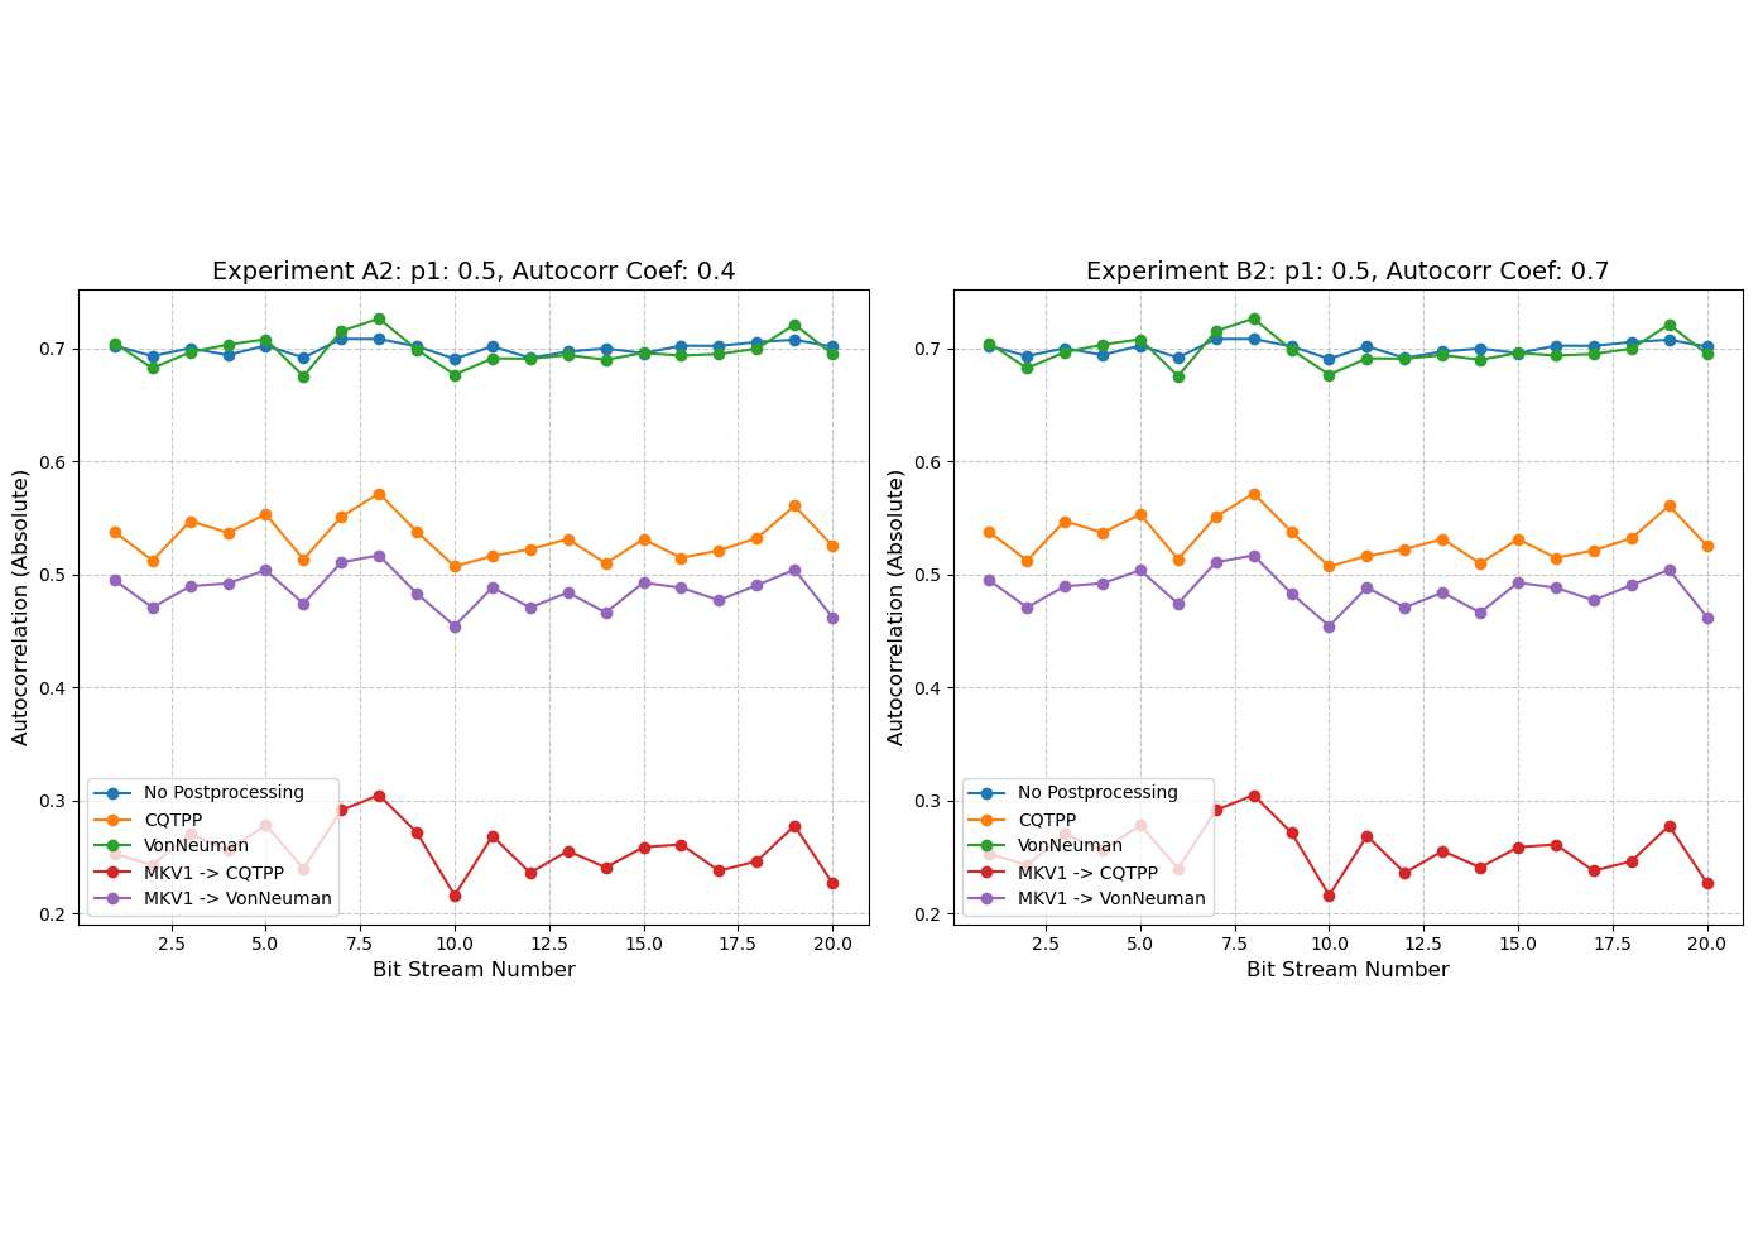
\includegraphics[width=\textwidth]{figures/AutoCorr.pdf}
    \caption{Autocorrealtion with lag k=1 in different bitsrreams using difernet post processors}
    \label{fig:grph4}
\end{figure}

\noindent for lag k = 2 we have results in \ref{fig:grph5}

\begin{figure}[h!]
    \centering
    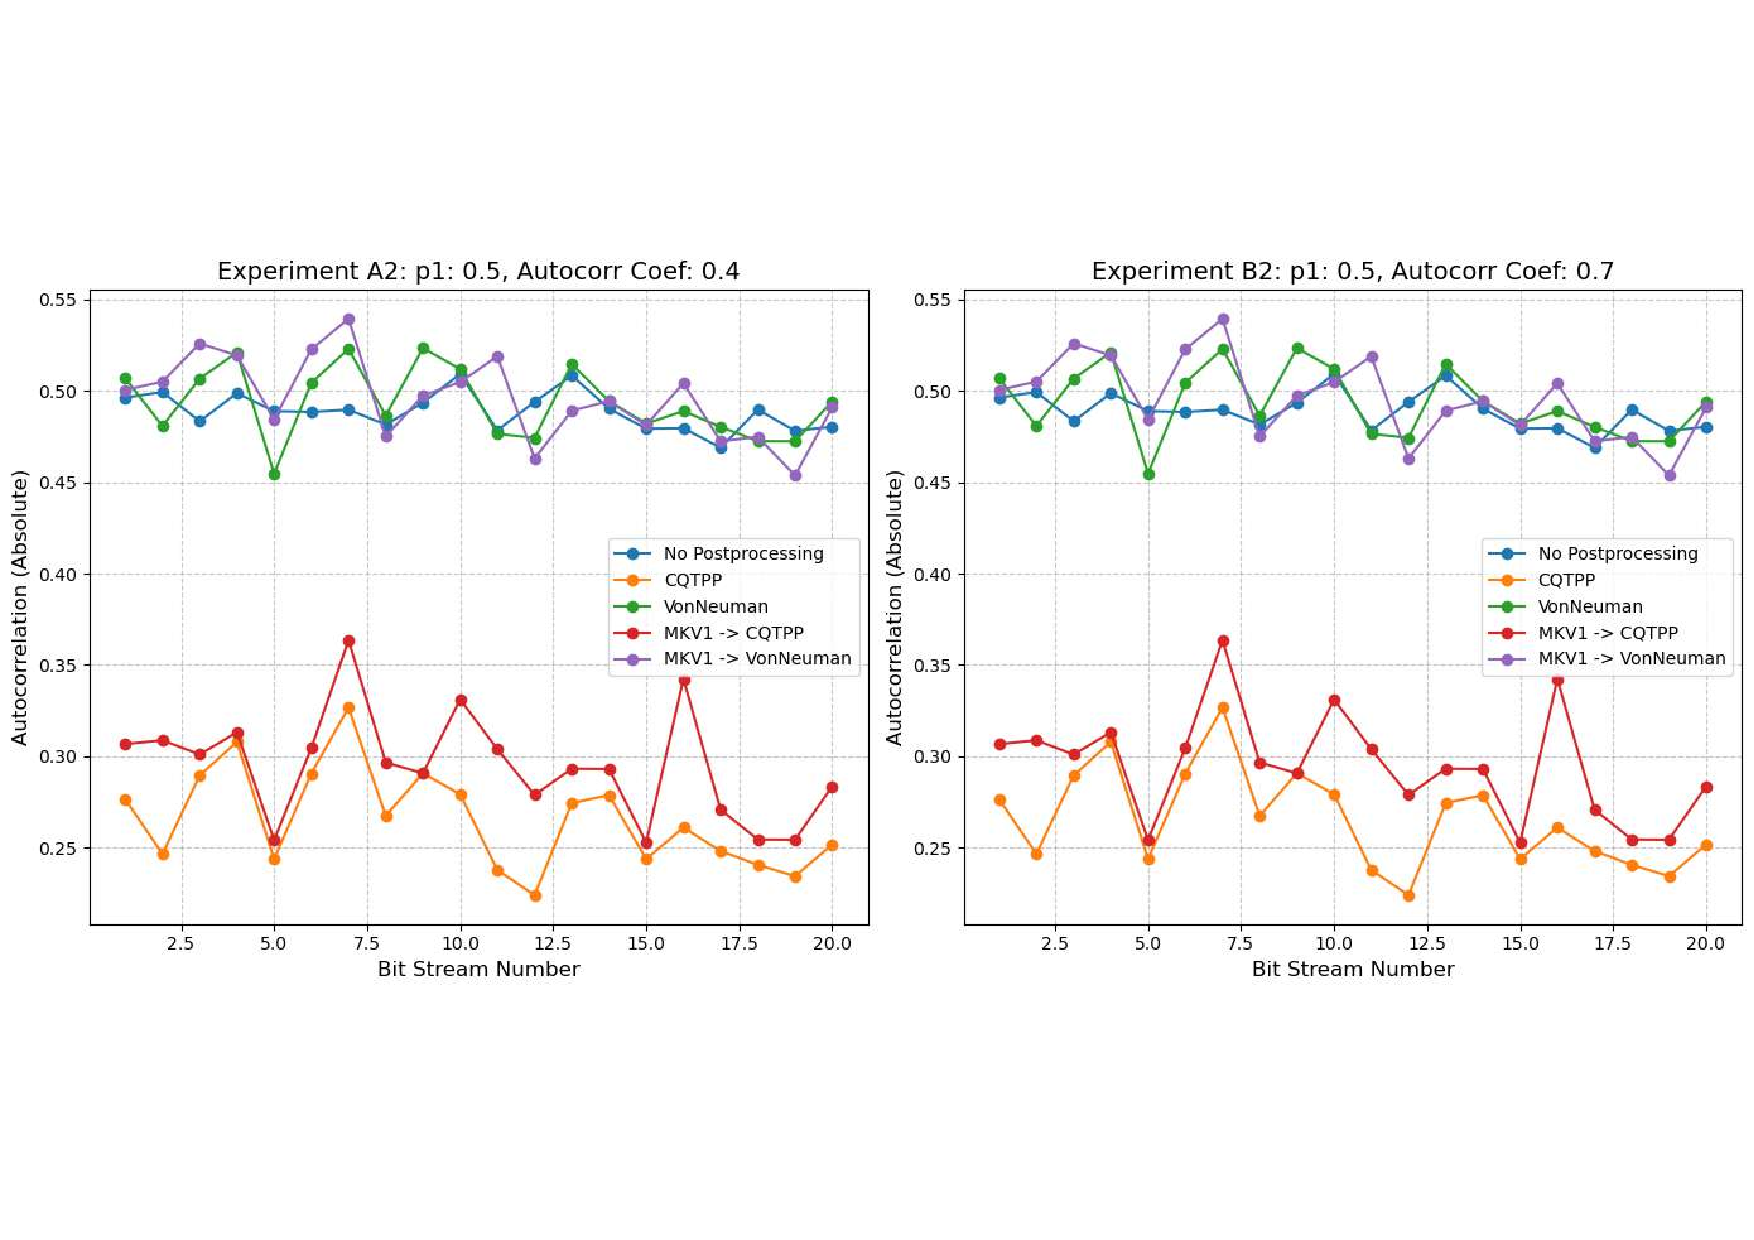
\includegraphics[width=\textwidth]{figures/AutoCorrLag2.pdf}
    \caption{Autocorrealtion with lag k=2 in different bitsrreams using difernet post processors}
    \label{fig:grph5}
\end{figure}

We can see from the results that the CQTPP+MKV achieves excellent results in decorrelating the input bitstream. The CQTPP achieves similar levels of decorrelation as the Von Neumann + MKV model, while the classical Von Neumann Post Processor gives the same autocorrelation results as the input.



\subsection{The Extraction Efficiency}

We calculated the extraction efficiency (ExE) of our post processors for different bitstream lengths. The results are shown in Fig. \ref{fig:grph6}.

\begin{figure}[h!]
    \centering
    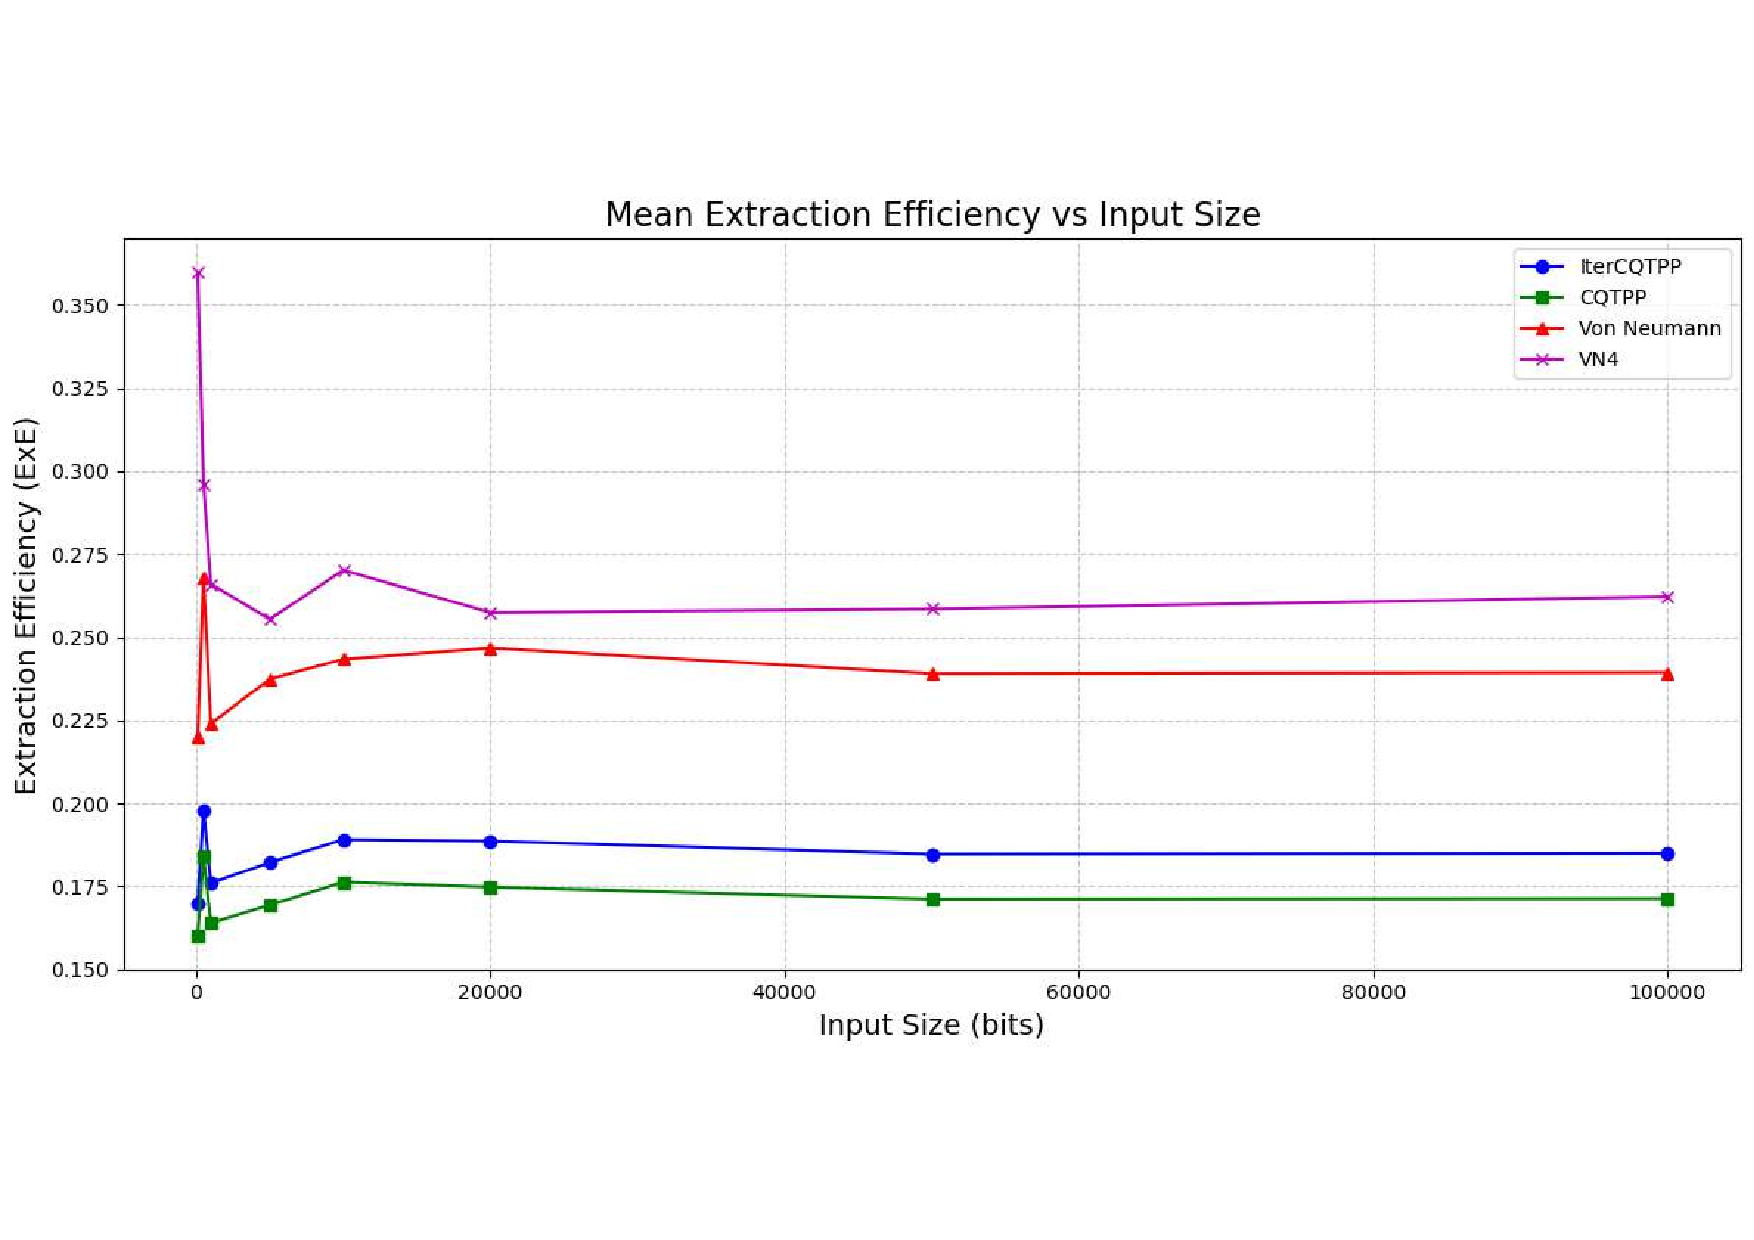
\includegraphics[width=\textwidth]{figures/ExE all.pdf}
    \caption{Extraction Efficiency (ExE) vs. Bitstream Length}
    \label{fig:grph6}
\end{figure}

Each of the post processors' ExE values converges to their theoretical ExE values. As we can see, the Von Neumann Post Processor with 4-bit chunks achieved the highest ExE. Meanwhile, the Iterative CQTPP (IterCQTPP) with 10 iterations provided slightly better results compared to the classical CQTPP.

Note: The combined post processors that include the Markov Chain were not included, since the Markov model does not affect the extraction rate of the bitstream.

\subsection{Remarks and Future Points to Be Exploited}

\textbf{1.} When working on exploring how to improve the throughput of the CQTPP, I noticed that there is a pattern of probabilities produced by the Von Neumann Post-Processor if we only look at the output of the same size. The CQTPP takes only the first bit, and by extracting the general pattern where the sum of the probabilities in sequences starting with the same bit and with the same length are equal (or converge to be so).

We can refine this further where I noticed that we could divide the output of VNPP that have the same length into three clusters, where if we take the sum of a portion of frequencies from each cluster, we can achieve similar probabilities without taking only the first bit. After reading the VN\_N technique \cite{zonga} more thoroughly, I think there might be some similarity between the proposed idea and it — though I’m not entirely sure. This point needs more work and investigation.

\textbf{2.} Another point that can also be exploited is to change the Von Neumann Post-Processor used in the CQTPP to one of its variants (We may use the VN\_8+Waiting strategy since it has a good rate according to \cite{zonga}). These variants will increase the rate of the Von Neumann output and, consequently, the rate of discarded bits produced by it in the CQTPP. Therefore, the Iterative CQTPP will significantly raise its throughput rate.